\section{Pisanje članka}
U teoriji novinar je borac za istinu, pa tragajući za njom, on sam bira teme koje će istraživati i na osnovu kojih će pisati članke. To je nikad dostignuti ideal istraživačkog novinarstva. U praksi je situacija drugačija i uglavnom su urednici ti koji odlučuju šta će određeni medij objaviti.
Tri su osnovna koraka medijskog rada:
\begin{enumerate}
\item prikupljanje informacija
\item obrada informacija
\item publikovanje informacija
\end{enumerate}

Kao i u svakoj firmi, u medijima postoje sastanci, tj. kolegijumi. Kolegijum je sastanak redakcije, dakle svih novinara i urednika. Na kolegijumu se raspoređuju dužnosti tako da svako od učesnika dobija oblast na kojoj će raditi. U velikim medijima, u kojima postoji nekoliko redakcija, svaka ima svoj kolegijum. Pored ovih pojedinačnih postoji i kolegijum svih redakcija, ali se on ređe održava. Naša izdavačka kuća još nije dostigla taj nivo da je potrebno više kolegijuma pa ćemo se baviti samo jednim kolegijumom kao jedinstvenim, što naravno ne znači da u budućnosti neće biti potrebe za više.
Kada je kolegijum završen sledi prikupljanje informacija. Prilikom prikupljanja in\-for\-ma\-ci\-ja, novinar treba da odgovori na čuvena \emph{5W1H} pitanja, tj. \\

\begin{itemize}
\item What happened?
\item Who is involved?
\item Where did it take place?
\item When did it take place?
\item Why did that happen?
\item How did it happen?
\end{itemize}

Novinar može da prikuplja informacije intervjuom, prevođenjem članaka i samostalnim istraživanjem. 
Prilikom obrade, novinar shodno svom stilu pakuje informaciju za objavljivanje. Obrada infromacija se sastoji od odvajanja bitnog od nebitnog, bilo koja da je vrsta materijala u pitanju: tekst, fotografije, audio ili video snimci. U obradi informacija novinaru pomažu lektor i dizajner. 

Objavljivanje(publikovanje) informacija se vrši novinar u dogovoru sa glavnim u\-red\-ni\-kom. Objavljivanje može usporiti ili osporiti cenzura. Cenzura može biti auto cenzura ili cenzura od strane glavnog urednika. \\


\begin{figure}[h]
    \centering
    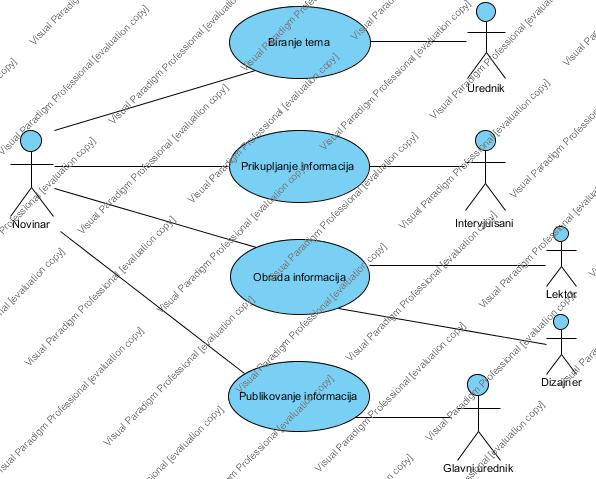
\includegraphics[width=0.7\textwidth]{slike/pisanje}
    \caption{Dijagram slučajeva upotrebe - pisanje članka}
    \label{pisanje}
\end{figure}

\subsection{Biranje tema (kolegijum)}

\begin{description}
\item [Opis] Novinari i urednici se dogovaraju oko tema koje će biti obrađene.
\item [Učesnici] Novinar, Urednik.
\item [Ulaz] Nema.
\item [Izlaz] Odabrane i dodeljene teme novinarima.
\item [Preduslovi] Dolazak dovoljnog broj novinara i urednika potrebnih za održavanje kolegijuma, prisustvo dovoljnog broj  novinara i urednika iz svake redakcije na kolegijumu.
\item [Postuslov] Uspešno odabrane i podeljene teme.
\end{description}      

\subsubsection{Glavni tok}
Urednici otpočinju kolegijum predstavljajući novinarima aktuelne teme i rezultate izvršenih analiza tržišta. Nakon izlaganja urednici daju reč novinarima. Novinar na osnovu svojih želja predlaže teme i traži odobrenje za istraživanje od urednika. Urednici zatim diskutuju o predloženim temama. Ukoliko se novinareve trenutne želje ne uklapaju sa vizijom urednika, urednici daju zadatke novinarima. Ukoliko se želje uklapaju u viziju urednika novinarev predlog se prihvata.
\subsubsection{Alternativni tok}
Ukoliko je potreban veći broj tema ili obrađivanje neke usko specijalizovane teme angažuju se honorarni novinari

\subsection{Prikupljanje informacija}
\begin{description}
\item [Opis] Novinar istražuje temu i piše prvu ruku članka.
\item [Učesnici] Novinar, Intervjuisani.
\item [Ulaz] Odabrane teme.
\item [Izlaz] Sirov(neobrađen) tekst.
\item [Preduslov] Ukoliko novinar vrši intervju, intervjuisana osoba je pristala na intervju.
\item [Postuslov] Tekst je uspešno napisan.
\end{description}      
\subsubsection{Glavni tok}
Novinar pregleda dobijene teme. Tema može da zahteva intervju, prevođenje ili samostalno istraživanje. Ukoliko tema zahteva intervju novinar zove osobu koju treba da intervjuiše. Intervjuisani u dogovoru sa novinarom može da prihvati ili odbije intervju. Ako je odbio intervju novinara, unosi u tekst informacije sa konstatacijom da intervju nije izvršen. Ukoliko prihvati intervju dogovara se sa novinarom o lokaciji i vremenu intervjua. Kada dodje na intervju novinar mu postavlja pitanja i snima odgovore. Kad se intervju završi novinar sa snimka zapisuje najzanimljivije. Ukoliko tema zahteva prevodjenje novinar preuzima tekst i prevodi ga. Ukoliko tema zahteva samostalno istraživanje novinar prikuplja literaturu, ako je potrebno organizuje neke manje intervjue. Na kraju iz hrpe prikupljenih informacija vadi najbitnije i zapisuje. 
\subsubsection{Alternativni tok}
U slučaju da kandidat odbije intervju, a drugi kandidat prihvati novinar može zanemariti prvog kandidata. 


\subsection{Obrada informacija}
\begin{description}
\item [Opis] Novinar, Lektor i Urednik proveravaju ispravnost članka.
\item [Učesnici] Novinar, Lektor, Urednik, Dizajner.
\item [Ulaz] Sirov(neobrađen) tekst.
\item [Izlaz] Tekst spreman za završnu obradu.
\item [Preduslov] Novinar je napisao neobrađeni tekst.
\item [Postuslov] Tekst je lektorisan i spreman za publikovanje.
\end{description}      
\subsubsection{Glavni tok}
Novinar čita tekst koji je napisao i važne delove, eventualno dopunjuje, u kontekstu onog što je trenutno aktuelno tj. onog što je vest. Kada je završio posao novinar predaje neobrađeni tekst lektoru. Lektor čita tekst i ukoliko primeti neke pravopisne, gramatičke i stilske greške vrši korekciju teksta. Čitanje i lektorisanje jednog teksta se vrši više puta. Kada je lektorisanje završeno, tekst se šalje uredniku da proveri istinitost konsultovanjem arhive ili više izvora. Ako je tekst istinit urednik ga odobrava u suprotnom tekst se odbacuje. Odobreni tekst salje se dizajneru koji dodaje slike, vrši prelome i stara se da tekst bude primamljiv oku. Kada je završio dizajner vraća tekst novinaru.
\subsubsection{Alternativni tok}
U borbi za čitaoce urednik se trudi da se informacija što pre objavi, pa se često preskaču koraci provere informacija i dolazi do objavljivanja neistinitih informacija.

\subsection{Publikovanje informacija}
\begin{description}
\item [Opis] Glavni urednik odobrava članak.
\item [Učesnici] Novinar, Glavni urednik.
\item [Ulaz] Obrađen tekst.
\item [Izlaz] Tekst spreman za objavljivanje i štampanje.
\item [Preduslov] Tekst je poslat uredniku.
\item [Postuslov] Tekst je odobrio urednik.
\end{description}      
\subsubsection{Glavni tok}
Novinar pregleda tekstove a zatim šalje tekst glavnom uredniku na odobrenje. Glavni urednik čita i analizira tekst. Ako glavni urednik nema zamerki, tekst dobija odobrenje da se šalje na internet objavljivanje i štampu. Ukoliko glavni urednik ima zamerki, tekst se šalje novinaru koji ga je pisao sa spiskom šta je potrebno da se uskladi. Upit može biti takav da se cenzuriše deo, čitav članak ili samo da se nešto doda. Ako je potrebno još dodati podataka ili novinar se vraća sa uputima urednika na koraka 3.1.2. Ako se cenzuriše čitav članak novinar odbacuje tekst, a ako se cenzuriše deo ide se na korak 3.1.3.
\subsubsection{Alternativni tok}
Ukoliko je ceo članak cenzurisan novinar može da pokuša da članak predstavi na sledećem kolegijumu 

	

\begin{figure}[h]
    \centering
    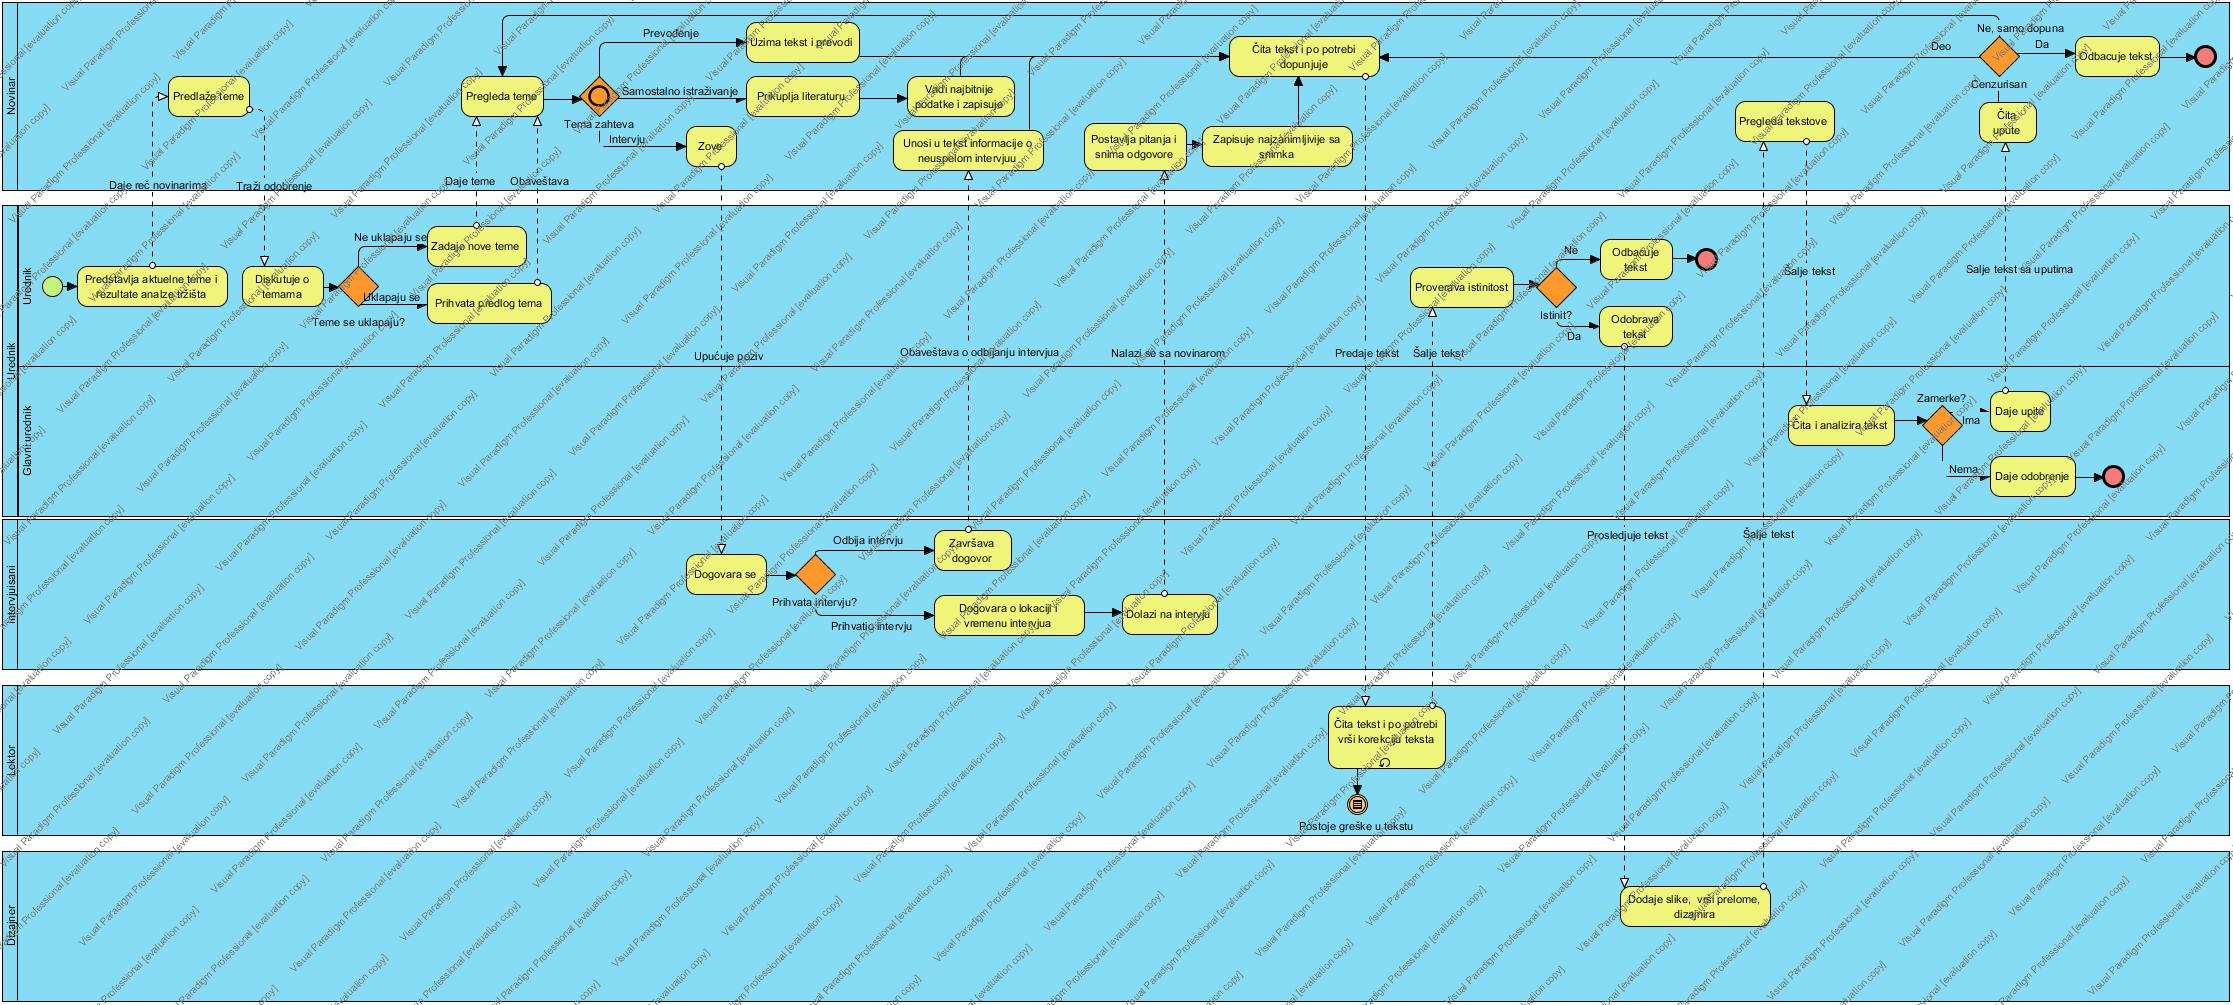
\includegraphics[width=1.0\textwidth]{slike/1-bpmn}
    \caption{BPMN dijagram}
    \label{pisanje}
\end{figure}	


.

\subsection{Komponovanje izdanja}
Za svako izdanje glavni i odgovorni urednik odlučuje o broju članaka. Takođe pored broja članaka se zna koliko kolor, a koliko crno-belih strana može izdanje da ima, kao i gde i koliko može oglasa da se nalazi. Nazalost pošto se danas novine i časopisi ne finansiraju samo od prodatih primeraka ili pretplatnika, već uglavnom od sponzora, za svakog novog sponzora, olgašivača mora da se nađe mesto, makar i na štetu kvaliteta sadržaja.

\subsubsection{Odabir članaka}
\begin{description}
\item [Opis] Glavni urednik bira članke koji će biti objavljeni.
\item [Učesnici] Glavni urednik.
\item [Ulaz] Članak spreman za objavljivanje i štampanje.
\item [Izlaz] Odabrani članci.
\item [Preduslov] Članak je spreman za objavljivanje i štampanje.
\item [Postuslov] Članak je poslat na štampu.
\end{description}   
\subsubsection{Glavni tok}
Glavni urednik pregleda članke. Pregled se sastoji od procene dužine, broja i kolora članaka. Ukoliko je broj, dužina ili kolor članaka veća od planirane vrši se odabir članaka. Ukoliko članci zadovoljavaju uslove, šalju se dalje na pripremu za štampu. Odabir članaka se vrši tako što prednost imaju aktuelne teme. 
\subsubsection{Alternativni tok}
Ukoliko je problem kolorit a sve teme su izuzetno aktuelne dozvoljava se u kontaktu sa menadžmentom da se prekorači dozvoljeni kolorit za najviše 5%.

\subsubsection{Smeštanje oglasa}
\begin{description}
\item [Opis] Glavni urednik smešta oglase u časopis.
\item [Učesnici] Glavni urednik, Oglašivač, Menadžment.
\item [Ulaz] Plaćeni oglasi.
\item [Izlaz] Raspoređeni oglasi.
\item [Preduslov] Oglašivač je platio mesto za oglas(e).
\item [Postuslov] Oglasi se nalaze na internet i/ili stampanom izdanju.
\end{description}   
\subsubsection{Glavni tok}
Glavni urednik sortira oglase prema važnosti (redovni sponzori, vanredni…). Kada je završio sa sortiranjem, urednik raspoređuje oglase prema veličini na unapred odabrane lokacije u časopisu. Ukoliko nema viška oglasa glavni urednik salje oglase na objavljivanje. Ukoliko ima više oglasa nego lokacija glavni urednik obaveštava menadžment koji onda kontaktira oglašivača. Oglašivač odlučuje da li će dodatno doplatiti da se njegov oglas nadje u časopisu na dodatnim stranama po unapred utvrđenom cenovniku ili će odustati. Ukoliko oglašivač prihvati ponudu, kad uplati sredstva kontaktira menadžment koji proverava uplatu i kontaktira glavnog urednika. Glavni urednik zatim izdaje naređenje da se oglas stavi na dodatnu stranu ili da se neki članak ukloni i na njegovo mesto dođe oglas. Ukoliko oglašivač odustane kontaktira se menadžment sa kojim se dogovara oko povraćaja novca
\subsubsection{Alternativni tok}
Ukoliko nema dovoljno oglasa raspisuje se kratkotrajni tender za prostor po smanjenoj ceni.

	
\begin{figure}[h]
    \centering
    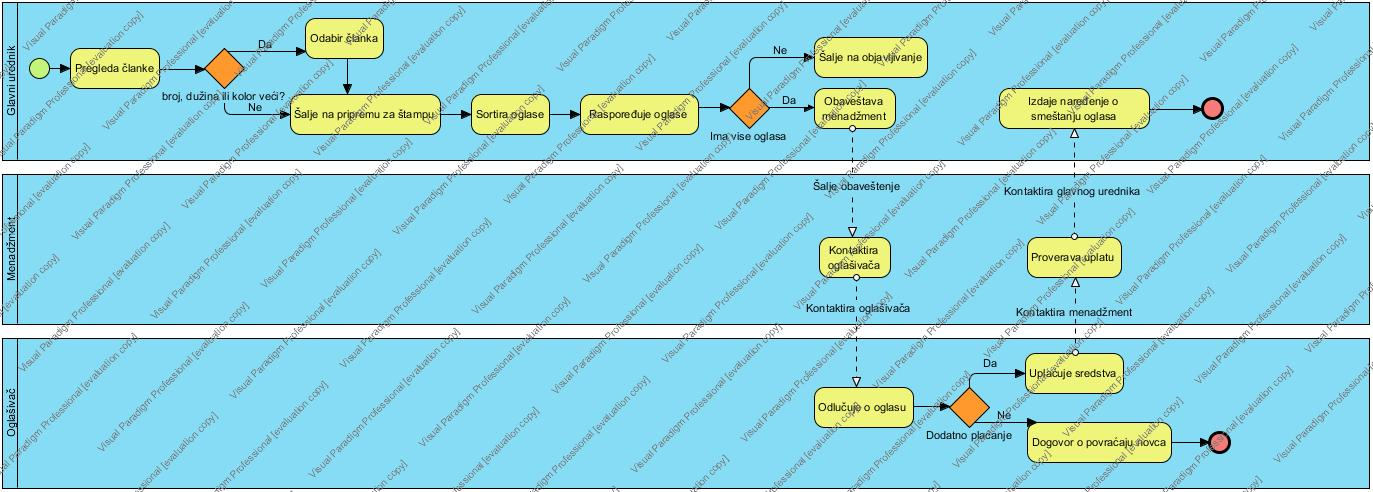
\includegraphics[width=1.0\textwidth]{slike/2-bpmn}
    \caption{BPMN dijagram}
    \label{pisanje}
\end{figure}	